\documentclass[border=10pt]{standalone}
\usepackage[svgnames]{xcolor}
\usepackage{amsmath}
\usepackage{pgfplots}
\pgfplotsset{compat=newest}
\usepackage[sfdefault]{FiraSans}
\usepackage{FiraMono}
\renewcommand*\familydefault{\sfdefault}
\begin{document}
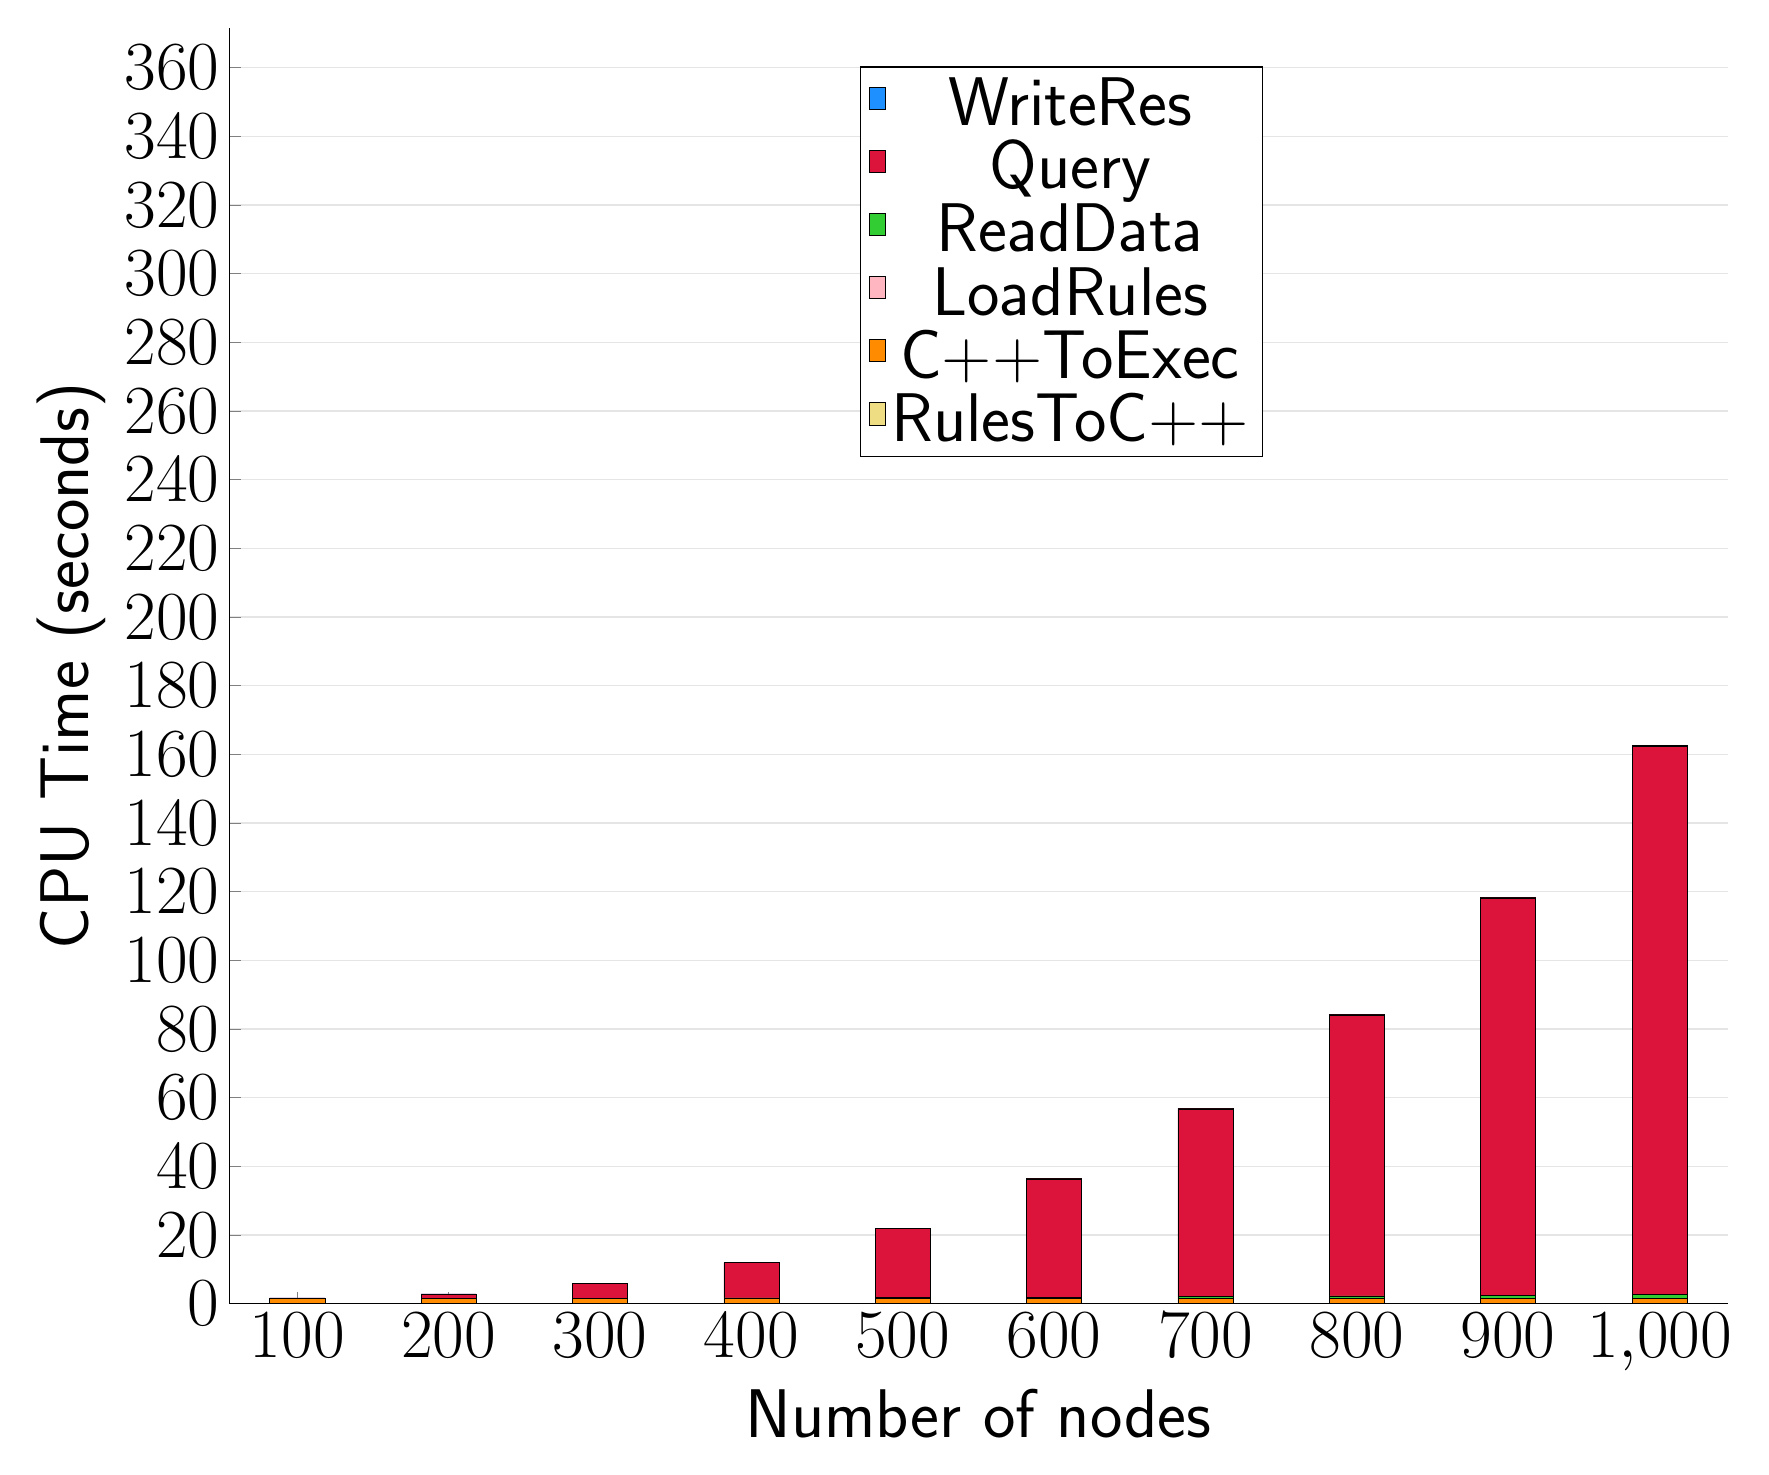
\begin{tikzpicture}
\begin{axis}[
   ybar stacked,
   width=1.7\textwidth,
   bar width=0.7cm,
   ymajorgrids, tick align=inside,
   major grid style={draw=gray!20},
   xtick=data,
   ymin=0, ymax=371.479,
   axis x line*=bottom,
   axis y line*=left,
   enlarge x limits=0.05,
   legend style={
       at={(0.69, 0.97)},
       anchor=north east,
       legend columns=1,
       font=\Huge,
   },
   ylabel={CPU Time (seconds)},
   xlabel={Number of nodes},
   label style={font=\Huge},
   tick label style={font=\Huge},
]
\addlegendimage{fill=DodgerBlue, draw=black, line width=0.2pt}
\addlegendentry{WriteRes}
\addlegendimage{fill=Crimson, draw=black, line width=0.2pt}
\addlegendentry{Query}
\addlegendimage{fill=LimeGreen, draw=black, line width=0.2pt}
\addlegendentry{ReadData}
\addlegendimage{fill=LightPink, draw=black, line width=0.2pt}
\addlegendentry{LoadRules}
\addlegendimage{fill=DarkOrange, draw=black, line width=0.2pt}
\addlegendentry{C++ToExec}
\addlegendimage{fill=LightGoldenrod, draw=black, line width=0.2pt}
\addlegendentry{RulesToC++}
\addplot +[fill=LightGoldenrod, draw=black, line width=0.2pt] coordinates {
(100, 0.010000000000000002)
(200, 0.008000000000000002)
(300, 0.0020000000000000005)
(400, 0.004000000000000001)
(500, 0.0)
(600, 0.0)
(700, 0.0)
(800, 0.0020000000000000005)
(900, 0.0)
(1000, 0.0)
};
\addplot +[fill=DarkOrange, draw=black, line width=0.2pt] coordinates {
(100, 1.478)
(200, 1.4780000000000002)
(300, 1.484)
(400, 1.482)
(500, 1.48)
(600, 1.474)
(700, 1.4759999999999998)
(800, 1.4739999999999998)
(900, 1.468)
(1000, 1.4680000000000002)
};
\addplot +[fill=LightPink, draw=black, line width=0.2pt] coordinates {
(100, 0.00012599999999999997)
(200, 0.00014319999999999998)
(300, 0.0001568)
(400, 0.00014680000000000002)
(500, 0.0001516)
(600, 0.00016199999999999998)
(700, 0.00016199999999999998)
(800, 0.0001752)
(900, 0.0001776)
(1000, 0.00016560000000000001)
};
\addplot +[fill=LimeGreen, draw=black, line width=0.2pt] coordinates {
(100, 0.0231698)
(200, 0.0680428)
(300, 0.123924)
(400, 0.20444279999999998)
(500, 0.3042548)
(600, 0.43476360000000003)
(700, 0.58579)
(800, 0.7591964)
(900, 0.9527090000000001)
(1000, 1.1774799999999999)
};
\addplot +[fill=Crimson, draw=black, line width=0.2pt] coordinates {
(100, 0.1734828)
(200, 1.288742)
(300, 4.2965919999999995)
(400, 10.239619999999999)
(500, 20.02356)
(600, 34.38988)
(700, 54.67282)
(800, 81.8471)
(900, 115.75139999999999)
(1000, 159.716)
};
\addplot +[fill=DodgerBlue, draw=black, line width=0.2pt] coordinates {
(100, 0.0023466)
(200, 0.008988600000000003)
(300, 0.019614600000000003)
(400, 0.0344806)
(500, 0.053383799999999995)
(600, 0.0766324)
(700, 0.104575)
(800, 0.1353092)
(900, 0.17125100000000001)
(1000, 0.2109734)
};
\end{axis}
\end{tikzpicture}

\end{document}
